%===================================== CHAP 2 =================================

\chapter{Ship Modelling and Control}
\section{Ship Model and Assumptions}

\subsection{Model Definition}
Normally, vessel dynamics are described with 6 degrees-of-freedom, with surge, sway and yaw describing position in the Cartesian 3-dimensional space, and roll, pitch and yaw as orientation variables around the axes. For a metacentrically stable ship in longitude and latitude, roll and pitch motions can be assumed zero, and since the ship is a surface vessel, we discard vertical position changes(the vessel is always at heave = 0). Thus, the maneuvering model is reduced to 3 DOF.

\begin{figure}[!h]
    \centering
    \includegraphics[width=0.75\textwidth]{fig/ship3dof.jpg}
    \caption{Ship degrees of freedom. Figure from \cite{ship3dof}}
    \label{fig:CSAD}
\end{figure}


The motion of a ship can be represented by the pose vector $\boldsymbol{\eta} = \left[ x ,y,\psi\right]^{\top} \in \mathbb{R}^2\times \mathbb{S}$ and the velocity vector $\boldsymbol{\nu} =\left[ u,v,r\right]^{\top}\in \mathbb{R}^3$.  Here, $(x,y)$ represents the Cartesian position in the local earth-fixed reference frame, $\psi$ is the yaw angle, $(u,v)$ represents the body-fixed linear velocities and $r$ is the yaw rate. The 3 DOF dynamics of a ship can then be stated based on the approach in \cite{fossen2011handbook} as:
\begin{align}
\boldsymbol{\dot{\eta}} &= \boldsymbol{R}(\psi)\boldsymbol{\nu}\label{eq:eta}\\
\boldsymbol{M\dot{\nu}}&+\boldsymbol{C(\nu)\nu}+\boldsymbol{D(\nu)\nu}=\boldsymbol{\tau},%+\mathbf{R}^{\top}(\psi)\boldsymbol{w},%+\omega^*},
\label{eq:nu}
\end{align}
where $\boldsymbol{M} \in \mathbb{R}^{3\times 3}$, $\boldsymbol{C(\nu)} \in \mathbb{R}^{3\times 3}$, $\boldsymbol{D(\nu)} \in \mathbb{R}^{3\times 3}$ and $\boldsymbol{\tau}= [\tau_1,\tau_2,\tau_3]^{\top}$
represent the inertia matrix, Coriolis and centripetal matrix, damping matrix and control input vector, respectively. The rotation matrix $\boldsymbol{R}(\psi) \in SO(3)$ is given by
\begin{align}
\boldsymbol{R}(\psi) &= \begin{bmatrix}
\cos(\psi) & -\sin(\psi) & 0\\
\sin(\psi) & \cos(\psi) & 0\\
0 & 0 & 1
\end{bmatrix}.
\end{align}
The system matrices are assumed to satisfy the properties $\boldsymbol{M} = \boldsymbol{M}{}^{\top}>0$, $\boldsymbol{C}(\boldsymbol{\nu}) = -\boldsymbol{C}(\boldsymbol{\nu})^{\top}$ and $\boldsymbol{D}(\boldsymbol{\nu}) >0$. 
%\\
%The parameter for the model ship CyberShip II from \cite{Skjetne2005} will be used populate the matrices for simulation purposes.\\

\begin{figure}[!h]
    \centering
    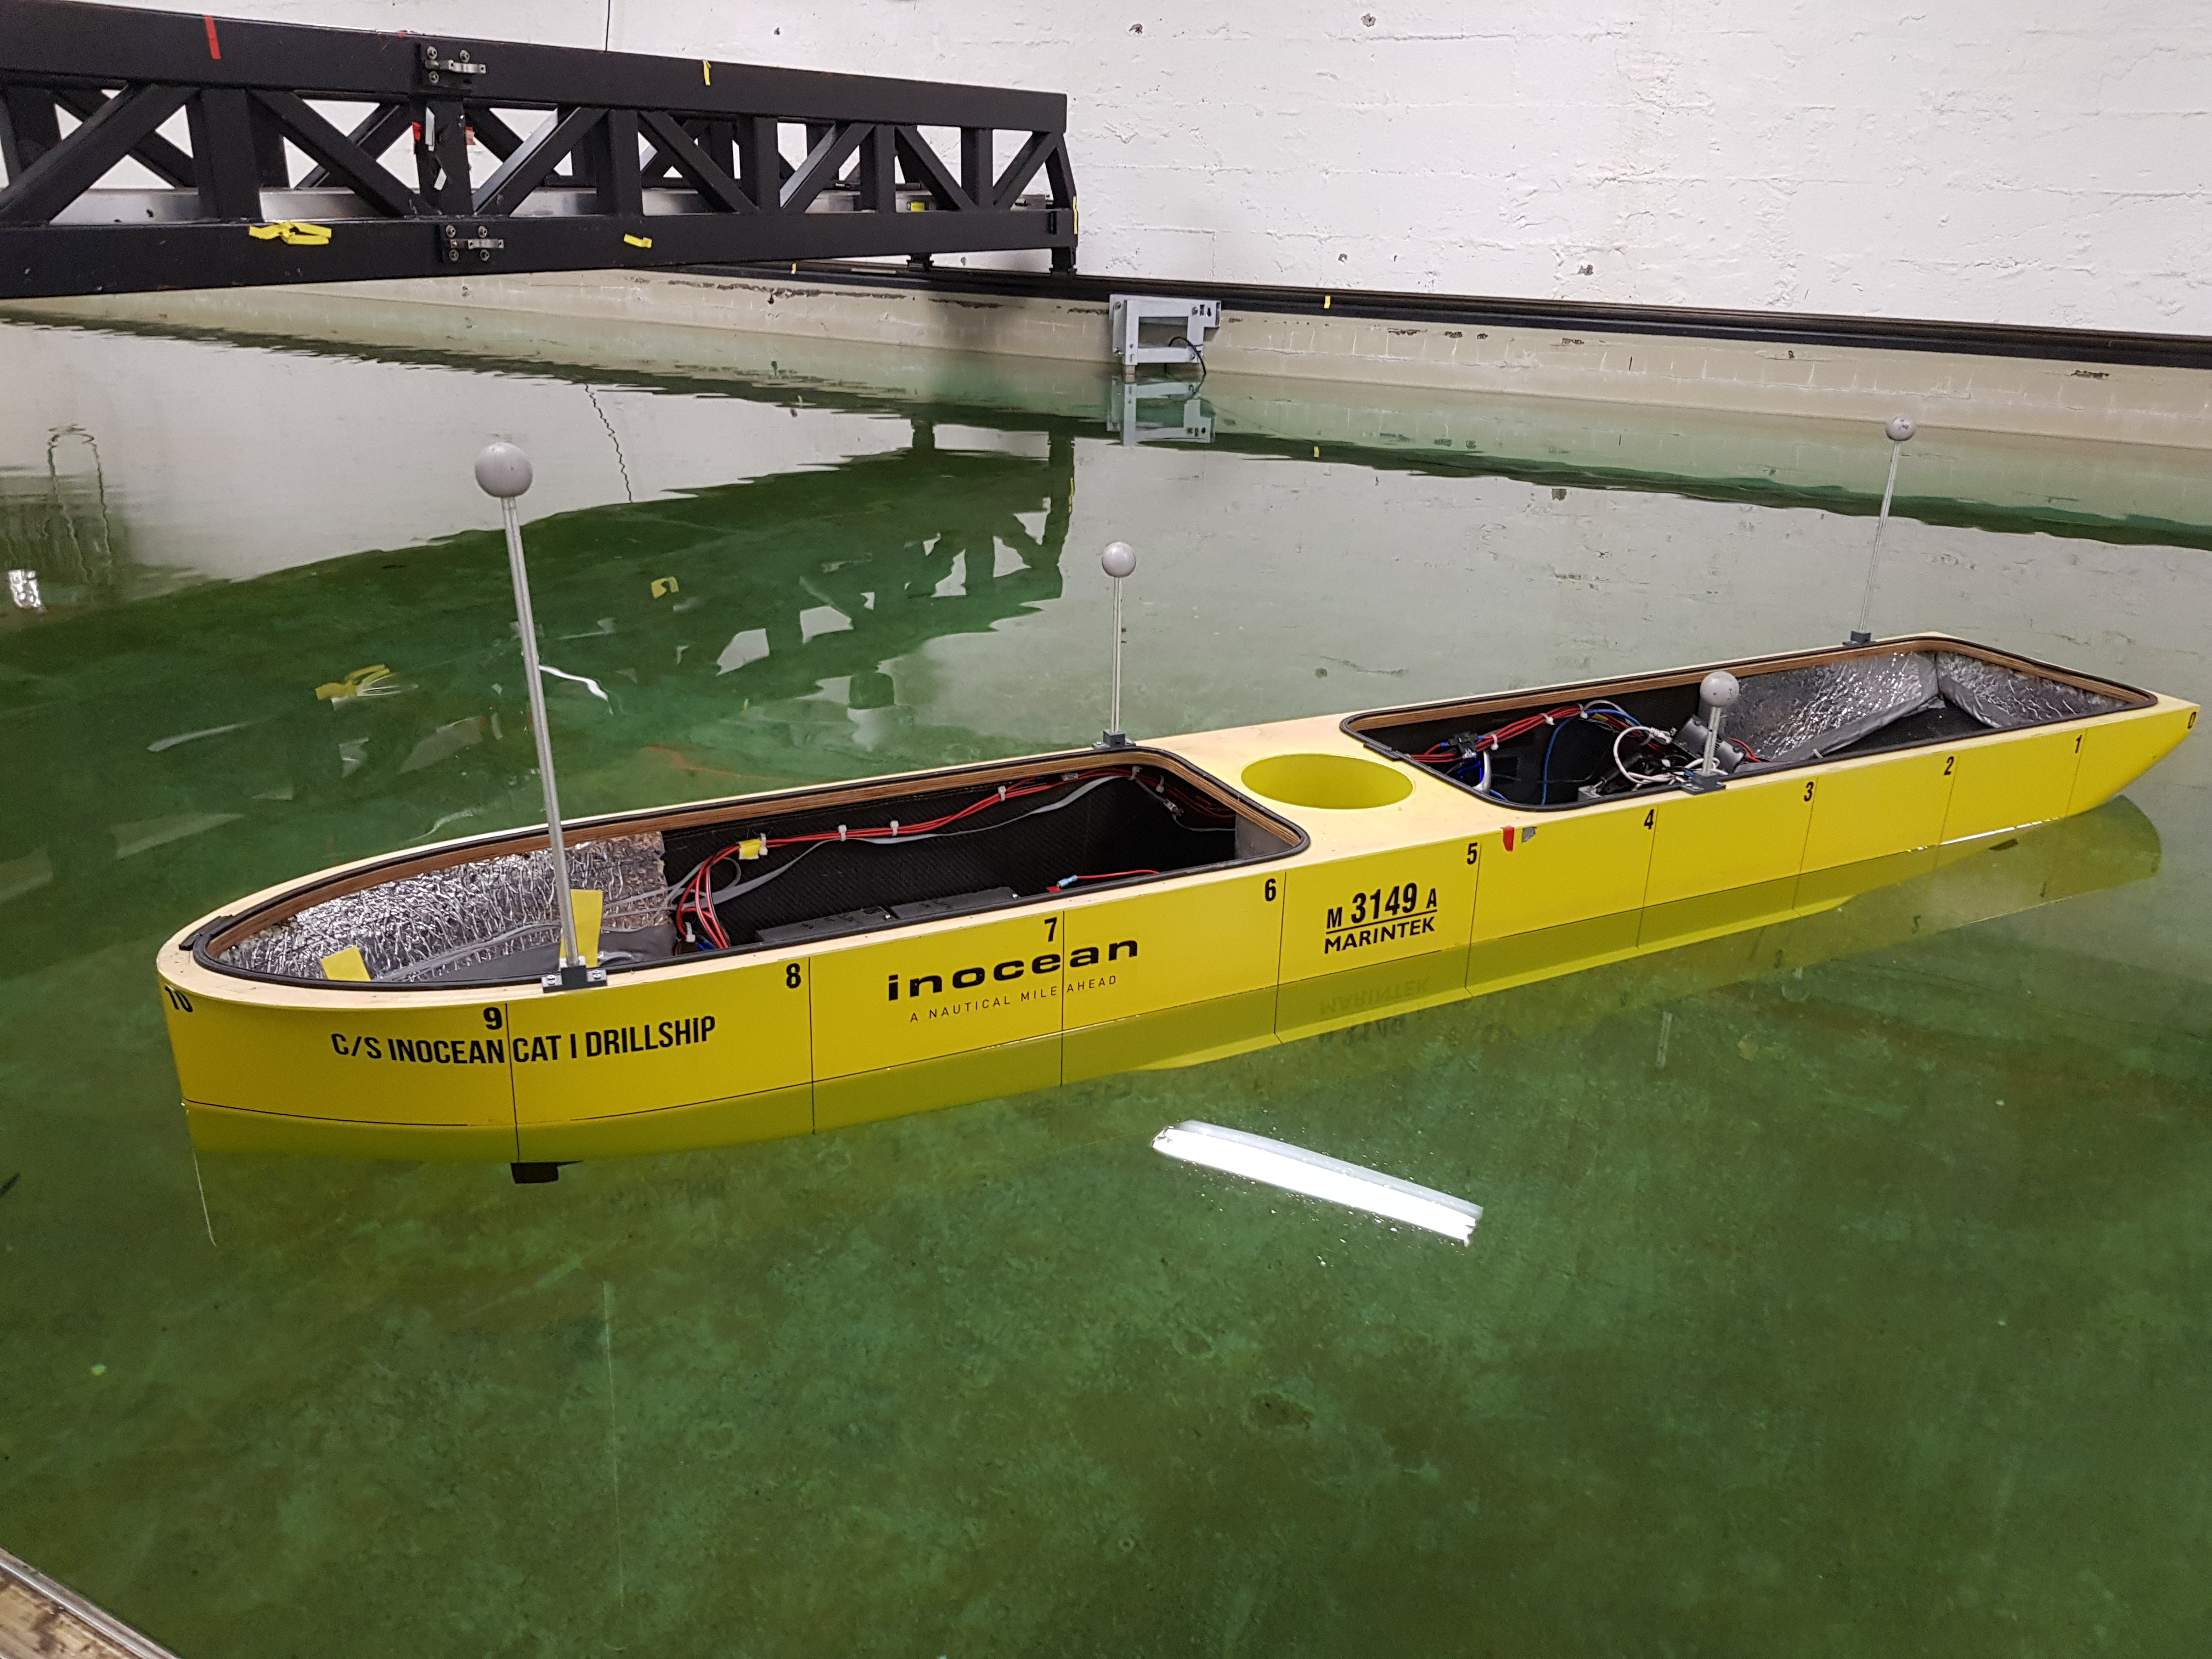
\includegraphics[width=0.65\textwidth]{fig/csad.jpg}
    \caption{C/S Inocean Cat I Drillship in the MC-lab.}
    \label{fig:CSAD}
\end{figure}


The model and parameters of the model-scale ship C/S Inocean Cat I Drillship \cite{bjorno}, hereafter abbreviated CSAD, is shown in Fig. \ref{fig:CSAD} and will be used in this thesis. CSAD is a 1:90 scale replica of a supply ship, with a length of $L = 2.578 ~\si{\meter}$.
The inertia matrix is given as
\begin{align}
\boldsymbol{M} = \boldsymbol{M}_{RB}+\boldsymbol{M}_{A},
\end{align}
where
\begin{align}
\boldsymbol{M}_{RB} &= \begin{bmatrix}
m & 0 & 0\\
0 & m & m x_g\\
0 & m x_g & I_z
\end{bmatrix}\\
 \boldsymbol{M}_A &= \begin{bmatrix}
-X_{\dot{u}} & 0 & 0\\
0 & -Y_{\dot{v}} & -Y_{\dot{r}}\\
0 & -N_{\dot{v}} & -N_{\dot{r}}
\end{bmatrix}.
\end{align}
CSAD has a mass of $m = 127.92 ~\si{\kilo\gram}$ and inertia about $z$-axis in the BODY-frame $I_z =  61.987 ~\si{\kilo\gram\meter\squared}$, while $x_g =  0.00375 ~\si{\meter}$ is the distance along the $x$-axis in the body frame from the centre of gravity. The full list of parameter values are shown in Table \ref{CSADParameters}.

The Coriolis and centripetal matrix is given as
\begin{equation}
\boldsymbol{C}(\boldsymbol{\nu}) = \boldsymbol{C_{RB}}(\boldsymbol{\nu}) + \boldsymbol{C_A}(\boldsymbol{\nu}),
\end{equation}
where
\begin{equation}
\boldsymbol{C_{RB}}(\boldsymbol{\nu}) = 
\begin{bmatrix}
0 & 0 & -m(x_gr + v)\\
0 & 0 & mu\\
m(x_gr + v) & -mu & 0
\end{bmatrix}
\end{equation}
\begin{equation}
\boldsymbol{C_{A}}(\boldsymbol{\nu}) = 
\begin{bmatrix}
0 & 0 & -c_{A,13}(\boldsymbol{\nu})\\
0 & 0 & c_{A,23}(\boldsymbol{\nu})\\
c_{A,13}(\boldsymbol{\nu}) & -c_{A,23}(\boldsymbol{\nu}) & 0
\end{bmatrix},
\end{equation}
where
\begin{align}
c_{A,13}(\boldsymbol{\nu}) &= -Y_{\dot{v}}v - Y_{\dot{r}}r\\
c_{A,23}(\boldsymbol{\nu}) &= -X_{\dot{u}}u.
\end{align}
\newline
Finally, the damping matrix $\boldsymbol{D}(\boldsymbol{\nu})$ is given as
\begin{equation}
\label{D1_nomod}
\boldsymbol{D}(\boldsymbol{\nu}) = \boldsymbol{D_L} + \boldsymbol{D_{NL}}(\boldsymbol{\nu}),
\end{equation}
where
\begin{equation}
\label{D_L_eq}
\boldsymbol{D_L} = 
\begin{bmatrix}
-X_u & 0 & 0\\
0 & -Y_v & -Y_r\\
0 & -N_v & -N_r
\end{bmatrix}
\end{equation}
\begin{equation}
\boldsymbol{D_{NL}}(\boldsymbol{\nu}) = 
\begin{bmatrix}
d_{NL,11}(\nu) & 0 & 0\\
0 & d_{NL,22}(\boldsymbol{\nu}) & d_{NL,23}(\boldsymbol{\nu})\\
0 & d_{NL,32}(\boldsymbol{\nu}) & d_{NL,33}(\boldsymbol{\nu})
\end{bmatrix},
\end{equation}
where
\begin{align}
d_{NL,11}(\boldsymbol{\nu}) &= -X_{|u|u}|u| - X_{uuu}u^2\\
d_{NL,22}(\boldsymbol{\nu}) &= -Y_{|v|v}|v|-Y_{|r|v}|r| - Y_{vvv}v^2\\
d_{NL,23}(\boldsymbol{\nu}) &= -Y_{|r|r}|r|-Y_{|v|r}|r| - Y_{rrr}r^2 - Y_{ur}u\\
d_{NL,32}(\boldsymbol{\nu}) &= -N_{|v|v}|v|-N_{|r|v}|v| - N_{vvv}v^2 - N_{uv}u\\
d_{NL,33}(\boldsymbol{\nu}) &= -N_{|r|r}|r|-N_{|v|r}|v| - N_{rrr}r^2 - N_{ur}u.
\end{align}
 
Where, in order to successfully accommodate for the Munk moment, the damping terms
\begin{align}
Y_{ur} &= -X_{\dot{u}}\\
N_{uv} &= - (Y_{\dot{v}} - X_{\dot{u}})\\
N_{ur} &= -Y_{\dot{r}},
\end{align}
which, when multiplied with $u$, are linearly increasing with the forward speed, are added to the damping matrix. This will result in a more physically realistic model behaviour, and will ensure that the model will not give rise to a physically impossible motion. \\
\begin{table}[h!]
\centering 
\begin{tabular}{| p{2cm} | p{2cm} | p{3cm} | p{2cm}|}
\hline
\textbf{Parameter}& \textbf{Bj\o rn\o2017 parameters \cite{bjørnø2017}} &  \textbf{New parameters} &\textbf{Unit}   \\ \hline\hline
$L$ & $2.578$ & $2.578$ & $m$  \\ \hline
$m$ & $127.92$ &127.92 & $kg$ \\ \hline
$x_g$ & $0$ & $\boldsymbol{0.0375}$ & $m$  \\ \hline
$I_z$ & $62$& 62 & $kgm^2$  \\ \hline
$X_{\dot{u}}$ &$3.26$& $\boldsymbol{-3.26}$ & $kg $ \\ \hline
$Y_{\dot{v}}$ &$28.9$& $\boldsymbol{-28.9}$ & $kg$  \\ \hline
$Y_{\dot{r}}$ & $0.525$ & $\boldsymbol{-0.525}$ & $kgm$  \\ \hline
$N_{\dot{v}}$ &$0.157$ &$\boldsymbol{-0.157}$ & $kgm$ \\ \hline
$N_{\dot{r}}$ & $14$ &$\boldsymbol{-14}$ & $kgm^2$  \\ \hline
$X_u$ & $ -2.33$ &-2.33 &$kg/s$  \\ \hline
$X_{|u|u}$ & $0$ &0& $kg/m $ \\ \hline
$X_{uuu}$ & $-8.56$ & -8.56&$kgs/m^2$  \\ \hline
$Y_v$ & -4.67 &-4.67 &$kg/s$\\ \hline
$Y_{|v|v}$ & $0.398$ & $\boldsymbol{-0.398}$ & $kg/m$\\ \hline
$Y_{vvv}$ & $-313$ & -313& $kgs/m^2$\\ \hline
$N_v$ & $0$ & 0 &$kgm/s$\\ \hline
$N_{|v|v}$ & $-0.209$ &-0.209 & $kg/m$\\ \hline
$N_{vvv}$ & $0$&0 & $kgs/m^2$\\ \hline
$Y_r$ & $-7.25$ &-7.25 &$kgm/s$\\ \hline
$Y_{|r|r}$ & $-3.450$&-3.450 & $kg/m$\\ \hline
$Y_{rrr}$ & $0$&0 & $kgs/m^2$\\ \hline
$N_r$ & $-0.0168$ & $\boldsymbol{-7.141}$ &$kg/s$\\ \hline
$N_{|r|r}$ & $-0.0115$&$ \boldsymbol{-4.888} $& $kgm^2$\\ \hline
$N_{rrr}$ & $-0.000358$&$\boldsymbol{-0.152}$ & $kgs/m^2$\\ \hline
$N_{|v|r}$ & $0.08$&0.08 & $kg/m$\\ \hline
$N_{|r|v}$ & $0.08$& 0.08& $kg/m$\\ \hline
$Y_{|v|r}$ & $-0.845$ &-0.845 &$kg$\\ \hline
$Y_{|r|v}$ & $-0.805$ & -0.805&$kg$\\ \hline
\end{tabular}
\caption{Numerical values of the ship model parameters for CSAD.}
\label{CSADParameters}
\end{table}

The parameters in Table \ref{CSADParameters} that are marked in bold are the ones that differ from the latest article regarding the CSAD. In \cite{bjørnø2017}, the parameters in $\boldsymbol{M}_A$ were positive signed, which doesn't make sense as they relate to the added mass in the inertia matrix, resulting in "removed mass". It could be that the wrong signage was a typo or an error in convention. 

Furthermore, parameters $N_r$, $N_{|r|r}$ and $N_{rrr}$ relates to the yaw motion, and were found to be too small regarding the ships relative yaw, giving the model a maximum yaw rate of 8398 [deg/s].
These parameters had not been scaled according to a realistic yaw rate, which were found to be 5 [deg/s], based on the maximum rotation rate from experiments done at the MC-lab in November 2017. To approximate appropriate values for these parameters, the internal scalings are kept as in \cite{bjørnø2017}, with the higher order terms dependent on $N_r$, and the ship model is simulated with a constant maximal yaw-moment. The value of $N_r$ is then tuned until the model yields a yaw-rate of approximately 5 [deg/s]. The final parameter values are displayed in Table \ref{CSADParameters}, marked in bold.







\subsection{Assumptions and Uncertainties}


The kinematic model used in model-based control application is normally determined by approximations and estimations, and will never represent the real world exactly. This uncertainties present in this approximated model will influence the performance of the control system. To counter this effect, a parameterization of uncertainty in the model is introduced, and a adaptive scheme is designed to change the system on-line. As well as handling inherent uncertainties, robust adaptive control can also compensate for measurement noise and disturbances in the closed-loop control system.  

For the 3 DOF ship model used in this thesis, the following parameterization is used based on \cite{Sørensen2015}, giving the relation between real $\boldsymbol{M}^*$,$\boldsymbol{C}^*$,$\boldsymbol{D}^*$ and the considered matrices:
\begin{align}\label{eq:uncert}
\bm{M}^* &= \delta\boldsymbol{M} \\
\bm{C}^* &= \delta\boldsymbol{C(\nu)} \\
\bm{D}^* &= \sigma\boldsymbol{D(\nu)}. 
\end{align}
It is assumed that disturbance and measurement noise is present in the system. In addition, the uncertainty of the actuator system in relation to the control input is given as $\boldsymbol{\tau}^*$ = $\rho \boldsymbol{\tau}$.

For notational simplicity, the matrices $\boldsymbol{C(\nu)}$, $\boldsymbol{D(\nu)}$ and $\boldsymbol{R}(\psi)$ will be written as $\boldsymbol{C}$, $\boldsymbol{D}$ and  $\boldsymbol{R}$ throughout this thesis.

\section{Methods of Actuator Handling}

\subsection{Command Governor - CG}

\subsection{Magnitude-Rate-Saturation - MRS}

\section{Adaptive Control}


\subsection{$\mathcal{L}_1$ Adaptive Control}

The design procedure of an $\mathcal{L}_1$ adaptive scheme is usually approached in 2 stages; The first stage consists of the design of a state estimator and and predictor as well as laws for adaptation updates, whereas the second stage concerns the design of the control law. The $\mathcal{L}_1$ Adaptive control system is designed as a cascaded control system, in which a nominal controller will be augmented with the $\mathcal{L}_1$ architecture. The nominal controller is a cascaded feedback nonlinear pose and velocity type system, as presented in \cite{Sørensen2016}.



\subsubsection{Stage 1: State Predictor and Adaptation}
\noindent
The prediction errors is defined as:
\begin{align}\label{prederror}
\boldsymbol{\tilde{\eta} = \hat{\eta} - \eta} \\
\boldsymbol{\tilde{\nu} = \hat{\nu} - \nu},
\end{align}
with $\boldsymbol{\eta, \nu}$ being measured pose and velocity and $\boldsymbol{\hat{\eta}, \hat{\nu}}$ being the respective estimates. The state prediction dynamics are defined as 
\begin{align}
\dot{\hat{\eta}} &= \boldsymbol{L_1\tilde{\eta} + R\nu}\\
\dot{\hat{\nu}} &= \boldsymbol{L_2\tilde{\nu} + M^{-1}}(\boldsymbol{\tau + R}^T\boldsymbol{\hat{w_{\delta}}-C\nu}-\boldsymbol{D\nu}).
\end{align}


To design the adaptation laws, a positive definite CLF is proposed:
\begin{align}\label{eq:L1ABV1}
V_1 =  \frac{1}{2\gamma_{w_{\delta}}} \tilde{\boldsymbol{w}}_{\delta}^T\tilde{\boldsymbol{w}}_{\delta} + \frac{1}{2}\tilde{\boldsymbol{\eta}}^T\tilde{\boldsymbol{\eta}} + \frac{1}{2}\tilde{\boldsymbol{\nu}}^T\boldsymbol{M}\tilde{\boldsymbol{\nu}}
\end{align} 
Differentiation of $V_1$ w.r.t time gives 
\begin{align}\label{eq: L1V1dot}
\dot{V}_1 &=  \frac{1}{\gamma_{w_{\delta}}}\tilde{\boldsymbol{w}}_{\delta}\dot{\hat{\boldsymbol{w}}}_{\delta} -\tilde{\boldsymbol{\eta}}^T\boldsymbol{L_1}\tilde{\boldsymbol{\eta}}+ \tilde{\boldsymbol{\nu}}^T(-\boldsymbol{ML_2}\tilde{\boldsymbol{\nu}}+ \boldsymbol{\tau} + \boldsymbol{R}^T\boldsymbol{\tilde{w}_{\delta}} -\boldsymbol{D\nu}) \\
\dot{V}_1 &= -\tilde{\boldsymbol{\eta}}^T\boldsymbol{L_1}\tilde{\boldsymbol{\eta}} -\boldsymbol{\tilde{\nu}}^{T} \boldsymbol{ML_2\tilde{\nu}}+ \tilde{\boldsymbol{w}}_{\delta}^T(\frac{1}{\gamma_{w_{\delta}}}\dot{\hat{\boldsymbol{w}}}_{\delta}+\boldsymbol{R\tilde{\nu}}).
\end{align}
The next step is to choose a adaptation law that ensure a negative definite $\dot{V_1}$ for all $\boldsymbol{\eta}, \boldsymbol{\nu} \neq 0$. 
Choosing adaptation law
\begin{align}\label{eq:L1laws1}
\dot{\hat{\boldsymbol{w}}}_{\delta} &= -\gamma_{w_{\delta}}\boldsymbol{R\tilde{\nu}}.
\end{align}
Substituting \eqref{eq:L1laws1}, $\dot{V}_1$ becomes 
\begin{align}
\dot{V}_1 = -\tilde{\boldsymbol{\eta}}^T\boldsymbol{L_1}\tilde{\boldsymbol{\eta}} -\boldsymbol{\tilde{\nu}}^{T} \boldsymbol{ML_2\tilde{\nu}},
\end{align}which is negative definite. \\


\subsubsection{Stage 2: Control law}

The next part regards the design of the cascaded control law, based on the approach in \cite{Sørensen2016}. The control errors for both pose and velocity $\boldsymbol{z}_i, i\in (1,2)$ are defined as: 

\begin{align}\label{eq:Abz}
\boldsymbol{z_1} &= \boldsymbol{R^T}(\psi)(\boldsymbol{\eta - \eta_t})\\
\boldsymbol{z_2} &= \boldsymbol{\nu - \alpha}
\end{align}


The control law is developed through the use of Control Lyapunov functions. The first quadratic function candidate is defined as:









\subsection{Immersion and Invariance Adaptive Control}


\section{The 4-corner Maneuvering Test}

The main objective of the control system is to ensure $\boldsymbol{\Tilde{\eta}}(t) \defeq \boldsymbol{\eta}(t)-\boldsymbol{\eta}_t(t) \xrightarrow{} \boldsymbol{0}$ when $t \rightarrow{} \infty$. Furthermore, it is desirable to analyze the performance of the control system during different modes of motion. For this reason, a test compromised of different motions will be utilized, a "4-corner test", inspired by \cite{Skjetne2017}. The 4-corner test is shown in Figure \ref{fig:4corner}. In this test, the ship is moved to 4 different set-points, or "corners" of a square, testing different modes of motion required of a autonomous ship. The movements in the 4-corner test are:
\begin{itemize}
    \item Position change $2\, (m)$ straight North: positive surge-only movement.
    \item Position change $2\, (m)$ straight East:  sway-only movement in starboard direction.
    \item Heading change $45\, (deg)$ clockwise:  pure yaw motion, "turning test", while holding position.
    \item Position change $2\, (m)$ straight South:  coupled surge-sway movement while holding heading degree. 
    \item Position change $2\, (m)$ straight West and heading change $45\, (deg)$ counterclockwise: coupled surge-sway-yaw movement.
\end{itemize}

\begin{figure}[!h]
    \centering
    \includegraphics[width=0.75\textwidth]{fig/4corner.png}
    \caption{4-corner test, modified from \cite{Skjetne2017}}
    \label{fig:4corner}
\end{figure}

\section{Performance Metrics}



For analyzing performance of control systems, performance metrics are a useful tool when comparing different types of controllers. 
Firstly, the tracking error is defined as the norm of the pose error:
\begin{align*}
    e = \sqrt[]{\boldsymbol{\tilde{\eta}}^T\boldsymbol{\tilde{\eta}}},  \boldsymbol{\tilde{\eta}} = \boldsymbol{\eta} - \boldsymbol{\eta_t}
\end{align*}
Be aware that this is not an exclusive definition, as the error can be defined multiple ways, including cross-track and velocity-tracking error. Knowing this, the following types of metric are used: \\



The IAE metric is an unweighted integral of the error over time, and is a simple measure on how well the controller holds the desired pose throughout the motions.
\begin{equation}
IAE(e) = \int_{t_0}^{t} \left|e\right|d\tau .
\end{equation}
The IAEW metric the power consumption $P= \left|\left|\boldsymbol{\nu^{\top}\tau}\right|\right|$ is used to scale the IAE-metric, and takes the energy consumption, and consequently, the energy efficiency into account.
\begin{equation}
IAEW(e) = \int_{t_0}^{t} \left|e\right|d\tau\int_{0}^{t}Pd\tau.
\end{equation}\\

Finally, it is desirable to evaluate the rate of change in the commanded input, which is relevant to take into account when the desire is to reduce wear and tear on actuators. The IADC-metric is proposed in \cite{}, and is defined as 
\begin{equation}
IADC(\bar{\boldsymbol{\tau}}) = \int_{t_0}^{t} \left|\dot{\bar{\boldsymbol{\tau}}}(\gamma)\right|d\gamma,
\end{equation}\\
with $\bar{\boldsymbol{\tau}}(t) = \sqrt{\boldsymbol{\tau}_u^2+\boldsymbol{\tau}_v^2+\boldsymbol{\tau}_r^2}$.
\cleardoublepage